\section{Introduction}
$\alpha$\textit{NLG}(short for Abductive Natural Language Generation)~\citep{Bhagavatula2020Abductive} 
is a conditional text generation task that
assesses the generation ability of models on abductively inferencing the most plausible explanation given the context.
An illustration example is shown in Figure~\ref{fig:intro_example}. Given the observation
$O_1$ at time $t_1$ and observation $O_2$ at time $t_2 > t_1$, the model needs to generate a
plausible hypothesis $H$ that can consistently explain both of the observations.
$\alpha$\textit{NLI}(short for Abductive Natural Language Inference) poses the same challenge as $\alpha$\textit{NLG} to
a model, except that the task is framed in a \textit{discriminative} setting: Given two observations $O_1$ and $O_2$ 
and two possible explanation hypotheses $H_1$ and $H_2$, a model is expected to choose the most plausible one explanation. %\JQ{It is necessary to use O and H symbols here?}

\begin{figure}[t]
    \centering
    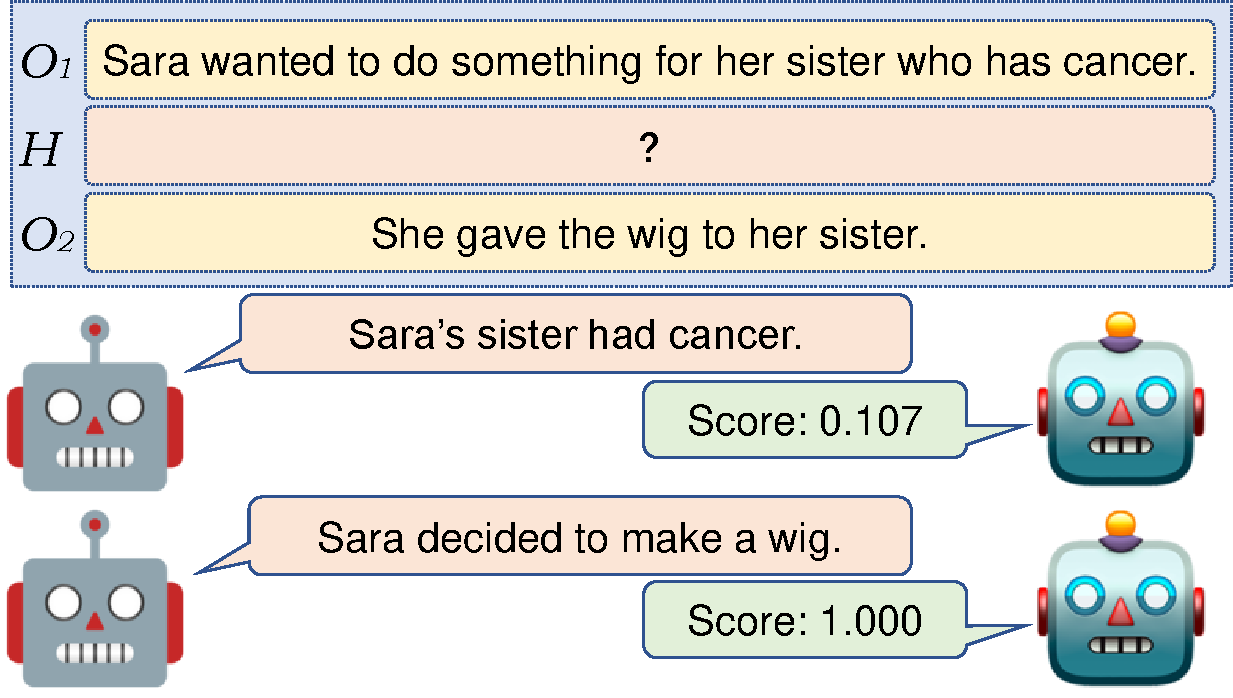
\includegraphics[width=1.0\columnwidth]{figs/intro_example.pdf}
    \caption{An illustration example of our intuition in $\alpha$\textit{NLG} dataset. Given the two observations
        $O_1$ and $O_2$, the generation model(on the left) need to compose a hypothesis that can consistently
        connect and explain both of the two observations. The teacher model(on the right)
        evaluates and gives a score to the generated hypothesis about how coherent and consistent it 
        is, thereby providing a explicit supervised signal for further training of the generative model.
    }
    \label{fig:intro_example}
\end{figure}

% Recent commonsense reasoning benchmarks, such as CommonsenseQA~\citep{commonsenseqa},
% SocialIQA~\citep{socialqa}, \textit{$\alpha$NLI}~\citep{Bhagavatula2020Abductive} and Story 
% Cloze Test(SCT) ~\citep{rocstory}, have been framed as \textit{discriminative} tasks in a 
% multi-choice setting, where model need to choose the most plausible answer among some candidates 
% according to the given context and the question. 
% To teach the model necessary background knowledge for addressing commonsense reasoning tasks,
% resorting to externel commonsense knowledge bases, such as ConceptNet ~\citep{conceptnet} and ATOMIC~\citep{atomic},
% and then combining the extracted and encoded knowledge subgraph with pre-trained language model~\citep{gpt2, bert, roberta}
% has been widely explored in \textit{discriminative} tasks~\citep{kagnet, lv, ye, connectingdots}.
% In \textit{generative} tasks, prevoius work~\citep{grf,Bhagavatula2020Abductive, DBLP:journals/tacl/GuanHHZZ20}
% incorporate knowledge into generative models by utilizing a similar extract-and-combine method.


% Commonsense \textit{generative} task is closely related to commonsense \textit{discriminative}
% task. On one hand, some commonsense benchmarks can be easily framed in both of \textit{generative} and
% \textit{discriminative} setting, like $\mathcal{ART}$($\alpha$\textit{NLG} + $\alpha$\textit{NLI})~\citep{Bhagavatula2020Abductive}
% and \textit{RocStory}(SEG + SCT)~\citep{rocstory}.
% On the other hand, they both essentially access the utilizing and reasoning ability
% over commonsense knowledge. However, previous work omits this point and solve these tasks independently.
% Another issue is that while previous work uses varied of methods to incorporate knowledge, the
% final training object is still the cross entropy loss, which cannot explicitly reflect the goal of 
% generating consistent and plausible text within the context following human commonsense knowledge.

 
% Existing work~\citep{l2r2, grf, backtofuture} solve these two tasks independently. %\JQ{add some details about previous work. such as: how well are the NLI performances while NLG is not very good ? and how did NLG train their model (like the plain log-likelyhood loss function?)}
To address $\alpha$\textit{NLG}, ~\citet{grf} resorted to external knowledge source~\citep{conceptnet,atomic}
and performed graph reasoning on a extracted knowledge subgraph to help geneartion.
~\citet{backtofuture} proposed an unsupervised decoding algorithm to incorporate the two observations.
Both of them solve $\alpha$\textit{NLG} independent of $\alpha$\textit{NLI}, ignoring the strong abductive
inferencing ability of a well-trained $\alpha$\textit{NLI} model.
Given the fact that both $\alpha$\textit{NLG} and $\alpha$\textit{NLI} investigate the same inference 
ability of models, we propose to boost the NLG performance by taking advantage of NLI models. 
With such a well-trained NLI model, the underlying objective of this task, i.e., the consistency and 
coherency of the generated hypothesis, can be using as a training target directly.

% \KZ{My main issue is that even if the EBM is better than the NLG model (GPT2 or BART), it does
% so by using much more data (double the amount?) I think the fair comparison with GPT2 or BART
% is by giving them the same amount of training data.}


%Given the fact that a well-trained $\alpha$\textit{NLI} 
%model can evaluate the consistency and coherency of the generated hypothesis from an $\alpha$\textit{NLG} model.
%If we can combine them in a teacher-student setting, we can train the $\alpha$\textit{NLG} model by the underlying task
%objective itself, insetad of the plain log-likelyhood loss function.

\begin{figure*}[ht]
    \centering
    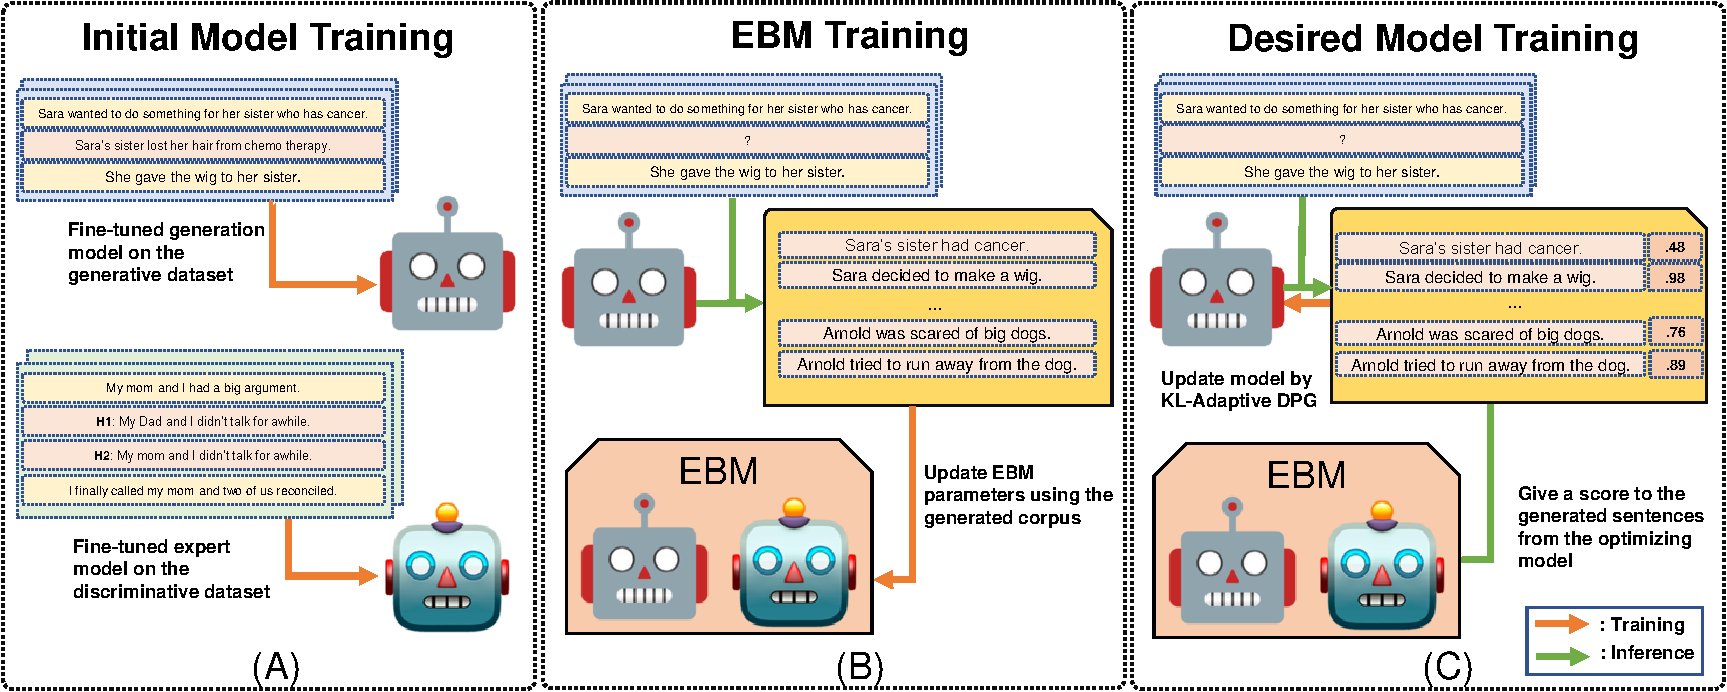
\includegraphics[width=1.0\textwidth]{figs/overview_graph.pdf}
    \caption{The training stages overview of our methods. 
    \textbf{(A)}: We firstly train the initial model $a$ on $\alpha$\textit{NLG} and $\phi(x)$ on $\alpha$\textit{NLI}.
    \textbf{(B)}: We sample sentences from $a$ as a corpus to train the EBM.
    \textbf{(C)}: The trained EBM scores each sentence generated by the policy model $q$ and instructs it
    for better generation. We implement this idea by formalizing the task in reinforcement learning setting
    and using the KL-Adaptive DPG algorithm.
    }
    \label{fig:overview}
\end{figure*}


To fullfill this intuition, we design our model under a teacher-student setting.
We firstly train a simple but good enough $\alpha$\textit{NLI} model as the teacher model
by fine-tuning a commonly-used pre-trained language model, such as BERT or RoBERTa~\citep{bert, roberta}.
Then we represent the desired optimal $\alpha$\textit{NLG} model as an Energy-Based Model~\citep{hintonebm,LeCun06atutorial,DBLP:conf/iclr/DengBOSR20}
with the teacher model and a base generation model~\citep{gpt2, bart}. % \JQ{not understand this sentence}
Finally, we train to reach the optimal $\alpha$\textit{NLG} model by the KL-Adaptive Distributional Gradient Policy algorithm.
% A series of expeirments are conducted to demonsrate and analyze the effectiveness of our proposed method. \JQ{show some specific results}
The best of our model outperforms the strong baseline models in varied evluation metrics, which
demonstrated the effectiveness and feasibility of our proposed method.

% To sum up, our work makes the following contributions:
% \begin{itemize}
%     \item We propose $\mathcal{COSER}$, a novel model solving commonsense generation tasks under 
%     the supervision of commonsense expert model.
%     \item We formulate the optimal desired generation model as a EBM model so that we can 
%     train the model explicitly by the ultimate goal of commonsense generation.
%     \item We conduct series of experiments to show the effectiveness of our proposed model, 
%     along with a complementary automatic evaluation metric.
% \end{itemize}

